% ===========================================================================
\subsection{Eight-piece hexagonal cavity: one Nb$_3$Sn wall}
% ===========================================================================

The first cavity was built in eight pieces so that every surface could be polished and coated flat (Fig.~\ref{fig:1stcavity}). That choice bought deposition uniformity and cost mechanical stiffness. Wall thickness fell below \qty{0.5}{\milli\meter} near the vertices, and the assembly contained eighteen copper-to-copper interfaces.

\begin{figure}[ht]
    \centering
    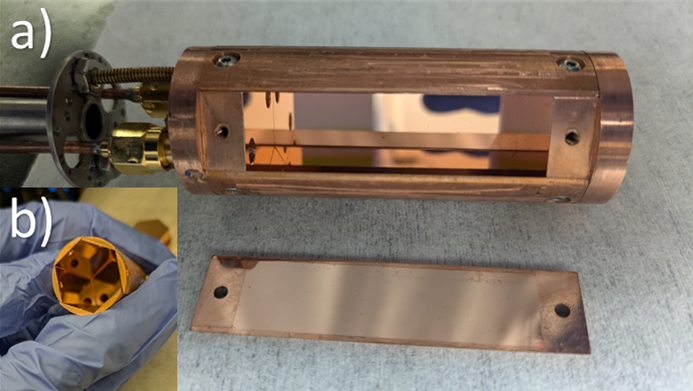
\includegraphics[width=0.75\linewidth]{images/AndreCavity/1stcavity.png}
    \caption{(a) Side view and (b) cross section of the eight-piece copper cavity: six walls and two endcaps.}
    \label{fig:1stcavity}
\end{figure}

Assembled bare with antenna couplers, the cavity gave $Q = 9{,}000$ at room temperature and $Q = 33{,}000$ ($R_s = \qty{11}{\milli\ohm}$) at \qty{4}{\kelvin}. Simulation of the same geometry with RRR-300 copper and no leakage predicts $Q = 13{,}500$ and $Q = 77{,}000$ ($R_s = \qty{5}{\milli\ohm}$) respectively. The cavity therefore reached \qty{43}{\percent} of its ideal cold $Q$, and squeezing the assembly changed the reading, which points at RF leakage through the eighteen interfaces rather than at the copper itself.

One of the six walls was then coated with Nb$_3$Sn by the Nb-first route (Fig.~\ref{fig:8pieceRecipe}). A custom holder gripped the wall at its top edge, where it mates with the endcap, leaving the interior face exposed. Inspection after reaction found film delamination near that gripped edge and at regions steeply inclined to the deposition flux (Fig.~\ref{fig:8pieceDelamination}) --- the first appearance of the coverage problem that recurs throughout this work.

\begin{figure}[ht]
    \centering
    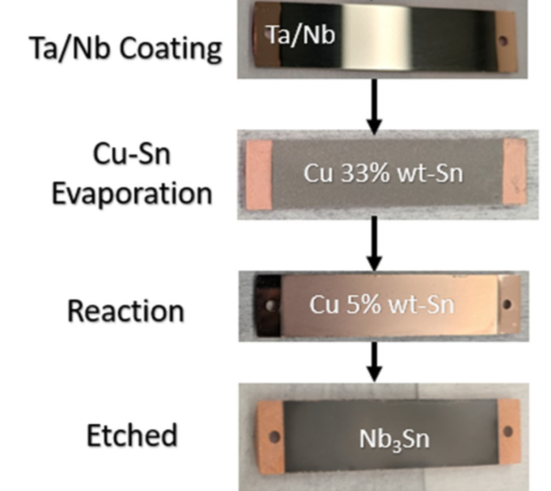
\includegraphics[width=0.75\linewidth]{images/AndreCavity/8pieceRecipe.png}
    \caption{Eight-piece cavity wall after the full Nb-first Nb$_3$Sn recipe.}
    \label{fig:8pieceRecipe}
\end{figure}

\begin{figure}[htb]
    \centering
    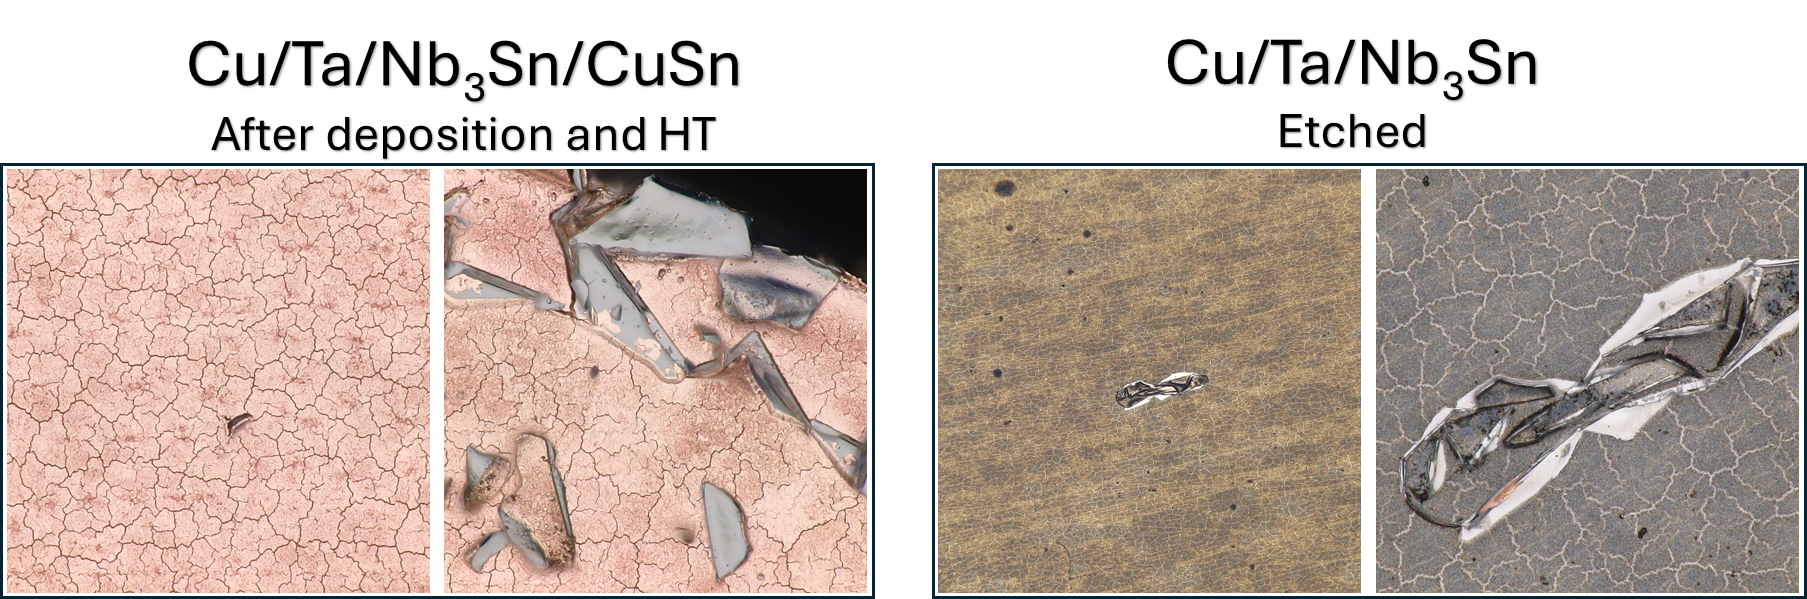
\includegraphics[width=\linewidth]{images/AndreCavity/8pieceDelamination.png}
    \caption{Delamination near the wall edge after heat treatment, shown before and after APS etching.}
    \label{fig:8pieceDelamination}
\end{figure}

\FloatBarrier

With one superconducting wall installed, $Q(T)$ showed a clear transition above the bare-copper baseline. Normalising the cavity surface resistance and overlaying it on the SQUID magnetisation curve of a coupon carried through the identical recipe puts both transitions at \qty{15}{\kelvin} (Fig.~\ref{fig:RSandMoment8Piece}). Transferring the recipe from a \qty{1}{\centi\meter} coupon to a cavity wall therefore produces the same material, which validates coupon $T_c$ as a process feedback metric for cavity work.

\begin{figure}[htb]
    \centering
    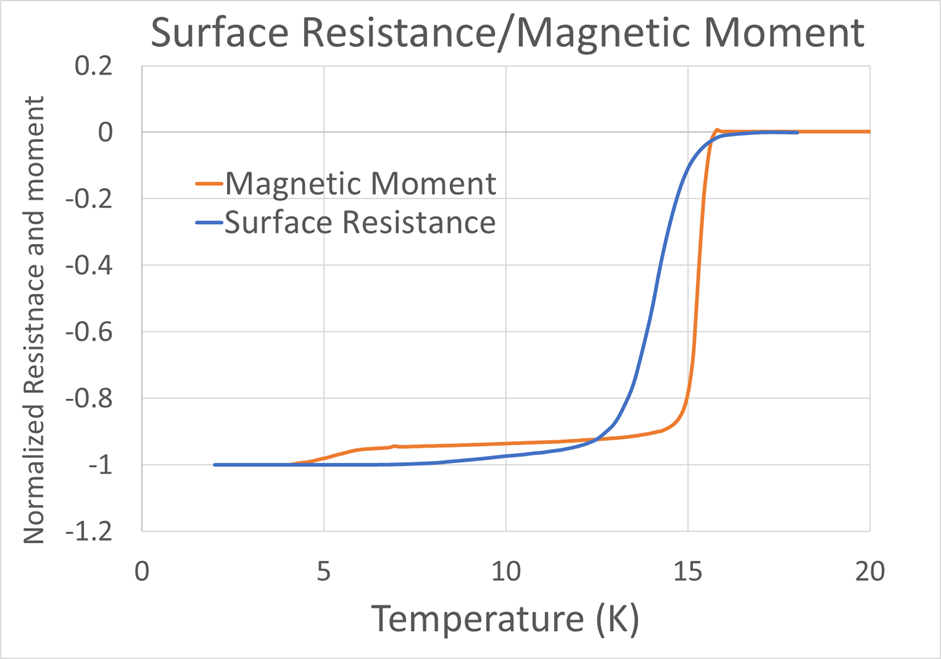
\includegraphics[width=0.5\linewidth]{images/AndreCavity/RSandMoment8Piece.png}
    \caption[Normalised cavity surface resistance compared with coupon SQUID magnetisation.]{Normalised cavity surface resistance compared with the SQUID magnetisation of a coupon from the same recipe. The agreement confirms that the cavity measurement senses the superconducting film.}
    \label{fig:RSandMoment8Piece}
\end{figure}

Isolating the coated wall requires subtracting the copper. Comparing the all-copper cavity with the one-superconducting-wall cavity, using the surface-specific geometric factors of Appendix~\ref{app:Qcorrection}, gives $R_s \approx \qty{8}{\milli\ohm}$ for the Nb$_3$Sn wall against \qty{11}{\milli\ohm} for copper (Fig.~\ref{fig:8pieceCavityRCorrected}). The transition appears at \qty{15}{\kelvin} and copper losses take over below about \qty{13}{\kelvin}. One wall out of eight surfaces is a small participation fraction, so the extracted value carries correspondingly large uncertainty.

\begin{figure}
    \centering
    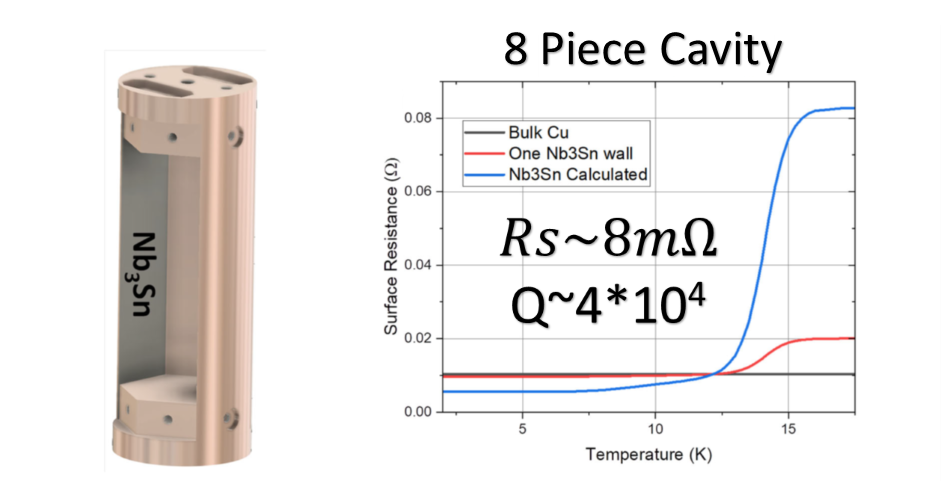
\includegraphics[width=0.9\linewidth]{images/AndreCavity/8pieceCavityRCorrected.png}
    \caption{Model of the eight-piece cavity with one Nb$_3$Sn wall, and $R_s(T)$ for bulk copper, the hybrid cavity, and the isolated superconducting wall.}
    \label{fig:8pieceCavityRCorrected}
\end{figure}

Field dependence was measured at \qty{2}{\kelvin} with the coated wall parallel to the applied field (Fig.~\ref{fig:8pieceQvsB}). $Q$ fell linearly with field and the superconducting state was lost near \qty{8}{\tesla}, far below the $H_{c2} > \qty{20}{\tesla}$ routine in Nb$_3$Sn wires. Below \qty{1}{\tesla} the superconducting wall was more resistive than bare copper. Geometry cannot explain this, because a wall parallel to the field should be the favourable orientation. The mechanism is discussed in Sec.~\ref{sec:discussion_field}.

\begin{figure}[htb]
    \centering
    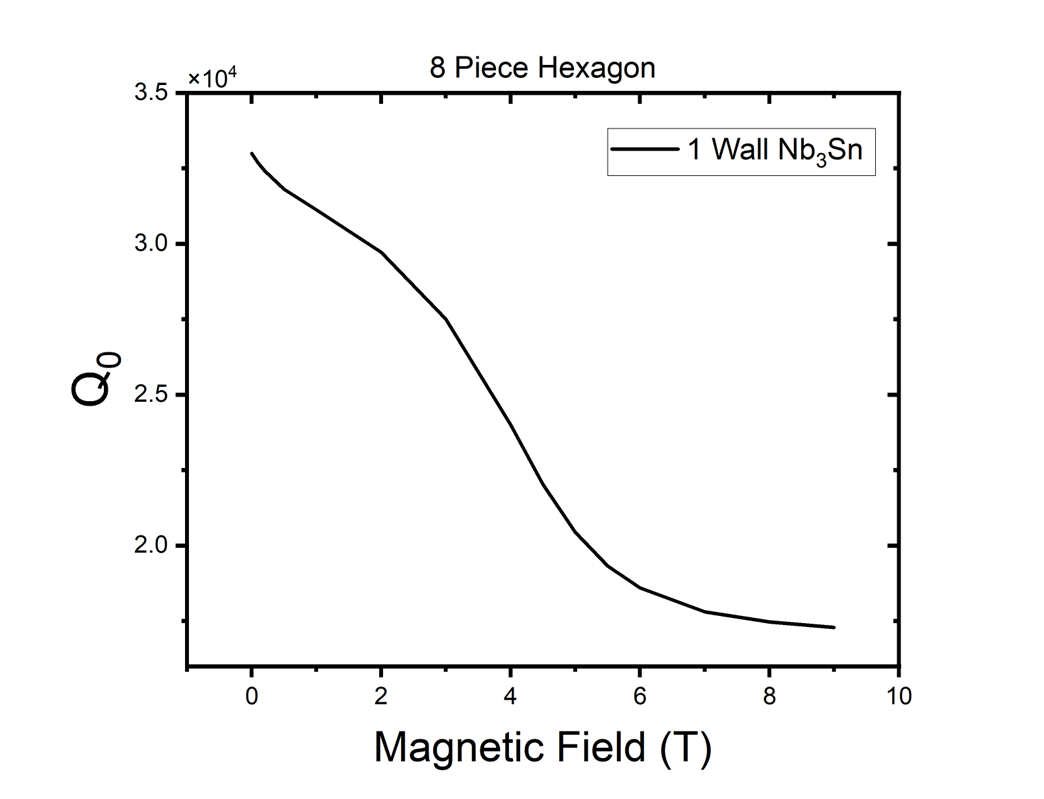
\includegraphics[width=0.75\linewidth]{images/AndreCavity/8pieceQvsB.png}
    \caption[Quality factor versus applied field for the single-wall eight-piece cavity.]{Quality factor versus applied magnetic field at \qty{2}{\kelvin} for the eight-piece cavity with one Nb$_3$Sn wall. The wall becomes normal conducting near \qty{8}{\tesla}.}
    \label{fig:8pieceQvsB}
\end{figure}

The prototype delivered its purpose. It established the measurement capability at ASC, it tied cavity RF data to coupon DC data, and it gave the first evidence that these films can beat copper. It also failed in two specific ways that set the next design: eighteen lossy interfaces, and severe $Q$ degradation in field. A version with six superconducting walls was not attempted, because the sub-millimetre vertices could not survive the assembly and thermal cycling that would require.
